% SIAM Article Template
\documentclass[review,onefignum,onetabnum]{siamart190516}
% SIAM Shared Information Template
% This is information that is shared between the main document and any
% supplement. If no supplement is required, then this information can
% be included directly in the main document.


% Packages and macros go here
\usepackage{lipsum}
\usepackage{amsfonts}
\usepackage{graphicx}
\usepackage{epstopdf}
\usepackage{algorithmic}
\ifpdf
  \DeclareGraphicsExtensions{.eps,.pdf,.png,.jpg}
\else
  \DeclareGraphicsExtensions{.eps}
\fi

% Add a serial/Oxford comma by default.
\newcommand{\creflastconjunction}{, and~}

% Used for creating new theorem and remark environments
\newsiamremark{remark}{Remark}
\newsiamremark{hypothesis}{Hypothesis}
\crefname{hypothesis}{Hypothesis}{Hypotheses}
\newsiamthm{claim}{Claim}

% Sets running headers as well as PDF title and authors
\headers{Application of semi-local sa to approximate pattern matching}{N. Mishin, and D. Berezun}

% Title. If the supplement option is on, then "Supplementary Material"
% is automatically inserted before the title.
\title{Application of semi-local sa to approximate pattern matching
  % \thanks{Submitted to the editors DATE.
  % \funding{This work was funded by the Fog Research Institute under contract no.~FRI-454.}}
}

% Authors: full names plus addresses.
\author{Nikita Mishin\thanks{Saint Petersburg State University, Russia
    (\email{mishinnikitam@gmail.com}).}
\and Daniil Berezun\thanks{IntelliJ Labs Co. Ltd., Saint Petersburg, Russia
  (\email{daniil.berezun@jetbrains.com}).}}

\usepackage{amsopn}
\DeclareMathOperator{\diag}{diag}


%%% Local Variables: 
%%% mode:latex
%%% TeX-master: "ex_article"
%%% End: 


% Optional PDF information
\ifpdf
\hypersetup{
  pdftitle={An Example Article},
  pdfauthor={D. Doe, P. T. Frank, and J. E. Smith}
}
\fi

% The next statement enables references to information in the
% supplement. See the xr-hyperref package for details.

\externaldocument{ex_supplement}

\newcommand{\red}[1]{\textcolor{red}{#1}}

\begin{document}

\maketitle

% REQUIRED
\begin{abstract}
  This is an example SIAM \LaTeX\ article. This can be used as a
  template for new articles.  Abstracts must be able to stand alone
  and so cannot contain citations to the paper's references,
  equations, etc.  An abstract must consist of a single paragraph and
  be concise. Because of online formatting, abstracts must appear as
  plain as possible. Any equations should be inline.
\end{abstract}


% REQUIRED
\begin{keywords}
  example, \LaTeX
\end{keywords}

% REQUIRED
\begin{AMS}
  68Q25, 68R10, 68U05
\end{AMS}

\section{Introduction}

% approximate string matching intro
The approximate pattern matching (\emph{AMatch}) is a well-known and studied problem.
Given some text $t$ and pattern  $p$ the \emph{AMatch} problem asks for all substrings of text $t$ that are close enough to pattern $p$ by some similarity measure.

% mant applications and difficulty
This problem arises in many fields such as computational biology, signal and image processing, text retrieval and etc \cite{}.
The diverse applications in sundry domains lead to different extensions of the problem which include additional constraints or even different objectives \cite{}.
Although there is a plurality of algorithms for solving the original \emph{AMatch} problem, the algorithm quantity dwindles notably when it comes to setting some constraints upon output.

The one such constraint naturally emerges and implicitly presented in various tasks\cite{TODO}. It refers to setting length bounds on matching substrings since minuscule or long matchings may be irrelevant to the subject of search (biologically insignificant, for example).
% Note that this constraint looks like

To the best of our knowledge, there is no formulation of extension of approximate pattern matching problem where the length of matchings explicitly limits, and, as consequences,  there is no study of this extended problem.

To close this gap, we take the liberty to define several extensions of \emph{AMatch} problem with explicitly set length constraint as well as provide algorithms for solving them. 
Recent achievements in RMQ in Monge matrices and novel \emph{semi-local lcs} problem is the key part of these algorithms.

We think that these problems with associated algorithms may be of practical use by virtue of natural constraints often occurring in different tasks.

In some ways, these algorithms are based on \cite{luciv2019interactive} algorithm.
In \cite{luciv2019interactive} the length constraint was given implicitly.
The algorithm is of interest not only because of the above limitation but also due to the fact that it satisfies some criteria of completeness that useful for some applications\footnote{the criteria is given in \cite{luciv2019interactive}}.
However, it has an unpleasant time complexity due to this limitation.

Taking into account the practical significance of \cite{luciv2019interactive}, we have developed an improved version of their algorithm with the perseverance of all of its properties based on the same concepts mentioned previously.

Thus, the main contribution of this paper is:
\begin{itemize}
    \item Improved version of the algorithm from \cite{luciv2019interactive}
    \item Definition and study of new extensions for  approximate pattern matching problem
    \item Algorithm for the new problem with an explicitly set length constraint on matching substrings 
\end{itemize}





% There also exist several variants of this problem that have different objectives with various implicitly or explicitly defined constraints.
% Although there are plenty of algorithms that solve \emph{AMatch} problem, the amount of algorithms significantly decreases when it comes to setting some constraints upon output. Nonetheless, recently, there was research in which the algorithm with implicitly defined length constraint was presented.
% This constraint was imposed on the lower and upper bound length of matching substrings.
% The algorithm is of interest not only because of the above limitation but also due to the fact that it satisfies some criteria of completeness that useful for some applications.
% However, it has an unpleasant time complexity.

% Taking into account the practical significance of this constraint in different tasks and domains we have developed an improved version of the algorithm [luciv] with the perseverance of all of its properties.
% This is achieved via adaptation and integration of algorithms that solve a novel string problem called "semi-local lcs problem".

% Further, we have defined a variant of \emph{AMatch} problem with explicitly set length constraint and presented exact and approximate algorithms for it.
% Recent achievements in RMQ in Monge matrices is the key part of these algorithms.

% Thus, the main contribution of this paper is:
% \begin{itemize}
%     \item Improved version of the algorithm from []
%     \item Algorithm for the new problem with an explicitly set length constraint on matching substrings 
%     \item Application of  "semi-local problem"
% \end{itemize}

\red{FILL WHEN OTHER PART IS READY}
The paper is orgranized as follows.

First, we give some basic definitions in section \ref{section:preliminaries}. Then, in  



% The length constraint of matching subsequences is an example of the latter one that often used in practice.
% It used in computational bioinformatics when the search  of a particular DNA subsequence in
% a large DNA sequence or DNA DATABASE is performed.
% Consider the case where we are given two matching substrings where the first one has a slightly higher similar score but has a significantly smaller size compared to the second one.
% There may be a situation when the application will yield only the first one substring although the second one may be more significant biologically.
% Thus, a specific lower bound on matching substrings should be set.

% Now consider the opposite case when the first one has a slightly smaller similar score but has a significantly smaller size compared to the second one.
% There could be a situation when the first one is much more significant in biology terms than the second one but the application will yield the second one. 
% Thus, a specific upper bound on matching substrings should be set.

% Same constraint arises in clone detection task when too small matching duplicates may be irrelevant  (article, interjections, punctuation marks, common words) whereas too big duplicates could not contains pattern at all (simply contains a word of pattern).


% The common approach of algorithm for approximate pattern matching utilizes  algorithm for solving the longest commons subsequence (\emph{LCS}) and sequence alignment (\emph{SA})  problems.

% The longest common subsequence is a well-known fundamental problem in computer science that also has many applications of its own.
% The major drawback of it that it shows only the global similarity for given input strings.
% For many tasks, it's simply not enough.
% The approximate matching is an example of it.

% There exist generalazation for \emph{LCS} called \emph{semi-local LCS}~\cite{tiskin2008semi} which can overcome this constraint. 
% The effective theoretical solutions for this generalized problem found applications to various algorithmic problems~\cite{tiskin2009periodic,tiskin2006longest,tiskin2011towards}.

% % research question Q1
% Although the algorithms for \emph{semi-local LCS} have good theoretical properties, there is unclear how they would behave in practice for a specific task and domain.
% More particularly, how it could be applied to approximate pattern matching with mentioned lower and upper bound on length constraint on matching subsequences.


% This paper is organized as follows

% % research question Q2
% To show the applicability of semi-local lcs on practice we developed several algorithms based mainly on it and the underlying algebraic structure.
% As well as developing new algorithms we improve the existing algorithm for duplicate detection in software documentation from~\cite{luciv2019interactive}.
% It should be noted that improvement preserves all properties of this algorithm.
% All presented algorithms also supports length constraints on the resulting substrings.
% Finally, we provided and proved running time and space complexity for all presented algorithms.





% Nonetheless, the number of suitable algorithms sharply decreases when the algorithm needs to meet some specific requirements imposed by running time, space complexity or specific criterion and constraints. 






% % short overview what constarins could be
% There exists a lot of algorithms that solve the above problem.
% Nonetheless, the number of suitable algorithms sharply decreases when the algorithm needs to meet some specific requirements imposed by running time, space complexity or specific criterion for the algorithm itself.
% For example, recently there was developed an approach for interactive duplicate detection for software documentation~\cite{luciv2019interactive}.
% The core of this approach is an algorithm that detects approximate clones of a given pattern $p$ with a specified degree of similarity and length boundaries for detected clones.
% The main advantage of the algorithm is that it meets a specific requirement of completeness.
% Nonetheless, it has an unpleasant time complexity.



   
% The common approach of algorithm for approximate detection utilizes mainly algorithm for solving the longest commons subsequence (\emph{LCS}) problem.

% The longest common subsequence is a well-known fundamental problem in computer science that also has many applications of its own.
% The major drawback of it that it shows only the global similarity for given input strings.
% For many tasks, it's simply not enough.
% The approximate matching is an example of it.

% There exist generalazation for \emph{LCS} called \emph{semi-local LCS}~\cite{tiskin2008semi} which overcome this constraint. 
% The effective theoretical solutions for this generalized problem found applications to various algorithmic problems~\cite{tiskin2009periodic,tiskin2006longest,tiskin2011towards}.
% %For example, there has been developed algorithm for approximate matching in the grammar-compresed strings~\cite{.}.

% % research question Q1
% Although the algorithms for \emph{semi-local LCS} have good theoretical properties, there is unclear how they would behave in practice for a specific task and domain.
% % research question Q2
% To show the applicability of semi-local lcs on practice we developed several algorithms based mainly on it and the underlying algebraic structure.
% As well as developing new algorithms we improve the existing algorithm for duplicate detection in software documentation from~\cite{luciv2019interactive}.
% It should be noted that improvement preserves all properties of this algorithm.
% All presented algorithms also supports length constraints on the resulting substrings.
% Finally, we provided and proved running time and space complexity for all presented algorithms.

% %% The paper is organized as follows.
% %% Blablabla
% %% \cref{sec:main}, our new algorithm is in \cref{sec:alg}, experimental
% %% results are in \cref{sec:experiments}, and the conclusions follow in
% %% \cref{sec:conclusions}.



\cref{sec:main}, our new algorithm is in \cref{sec:alg}, experimental
results are in \cref{sec:experiments}, and the conclusions follow in
\cref{sec:conclusions}.

\section{Main results}
\label{sec:main}

We interleave text filler with some example theorems and theorem-like
items.

\lipsum[4]

Here we state our main result as \cref{thm:bigthm}; the proof is
deferred to \cref{sec:proof}.

\begin{theorem}[$LDL^T$ Factorization \cite{GoVa13}]\label{thm:bigthm}
  If $A \in \mathbb{R}^{n \times n}$ is symmetric and the principal
  submatrix $A(1:k,1:k)$ is nonsingular for $k=1:n-1$, then there
  exists a unit lower triangular matrix $L$ and a diagonal matrix
  \begin{displaymath}
    D = \diag(d_1,\dots,d_n)
  \end{displaymath}
  such that $A=LDL^T$. The factorization is unique.
\end{theorem}

\lipsum[6]

\begin{theorem}[Mean Value Theorem]\label{thm:mvt}
  Suppose $f$ is a function that is continuous on the closed interval
  $[a,b]$.  and differentiable on the open interval $(a,b)$.
  Then there exists a number $c$ such that $a < c < b$ and
  \begin{displaymath}
    f'(c) = \frac{f(b)-f(a)}{b-a}.
  \end{displaymath}
  In other words,
  \begin{displaymath}
    f(b)-f(a) = f'(c)(b-a).
  \end{displaymath}
\end{theorem}

Observe that \cref{thm:bigthm,thm:mvt,cor:a} correctly mix references
to multiple labels.

\begin{corollary}\label{cor:a}
  Let $f(x)$ be continuous and differentiable everywhere. If $f(x)$
  has at least two roots, then $f'(x)$ must have at least one root.
\end{corollary}
\begin{proof}
  Let $a$ and $b$ be two distinct roots of $f$.
  By \cref{thm:mvt}, there exists a number $c$ such that
  \begin{displaymath}
    f'(c) = \frac{f(b)-f(a)}{b-a} = \frac{0-0}{b-a} = 0.
  \end{displaymath}
\end{proof}

Note that it may require two \LaTeX\ compilations for the proof marks
to show.

Display matrices can be rendered using environments from \texttt{amsmath}:
\begin{equation}\label{eq:matrices}
S=\begin{bmatrix}1&0\\0&0\end{bmatrix}
\quad\text{and}\quad
C=\begin{pmatrix}1&1&0\\1&1&0\\0&0&0\end{pmatrix}.
\end{equation}
Equation \cref{eq:matrices} shows some example matrices.

We calculate the Fr\'{e}chet derivative of $F$ as follows:
\begin{subequations}
\begin{align}
  F'(U,V)(H,K) 
  &= \langle R(U,V),H\Sigma V^{T} + U\Sigma K^{T} -
  P(H\Sigma V^{T} + U\Sigma K^{T})\rangle \label{eq:aa} \\
  &= \langle R(U,V),H\Sigma V^{T} + U\Sigma K^{T}\rangle 
  \nonumber \\
  &= \langle R(U,V)V\Sigma^{T},H\rangle + 
  \langle \Sigma^{T}U^{T}R(U,V),K^{T}\rangle. \label{eq:bb}
\end{align}
\end{subequations}
\Cref{eq:aa} is the first line, and \cref{eq:bb} is the last line.

\section{Algorithm}
\label{sec:alg}

\lipsum[40]

Our analysis leads to the algorithm in \cref{alg:buildtree}.

\begin{algorithm}
\caption{Build tree}
\label{alg:buildtree}
\begin{algorithmic}
\STATE{Define $P:=T:=\{ \{1\},\ldots,\{d\}$\}}
\WHILE{$\#P > 1$}
\STATE{Choose $C^\prime\in\mathcal{C}_p(P)$ with $C^\prime := \operatorname{argmin}_{C\in\mathcal{C}_p(P)} \varrho(C)$}
\STATE{Find an optimal partition tree $T_{C^\prime}$ }
\STATE{Update $P := (P{\setminus} C^\prime) \cup \{ \bigcup_{t\in C^\prime} t \}$}
\STATE{Update $T := T \cup \{ \bigcup_{t\in\tau} t : \tau\in T_{C^\prime}{\setminus} \mathcal{L}(T_{C^\prime})\}$}
\ENDWHILE
\RETURN $T$
\end{algorithmic}
\end{algorithm}

\lipsum[41]

\section{Experimental results}
\label{sec:experiments}

\lipsum[50]

\Cref{fig:testfig} shows some example results. Additional results are
available in the supplement in \cref{tab:foo}.

\begin{figure}[htbp]
  \centering
  \label{fig:a}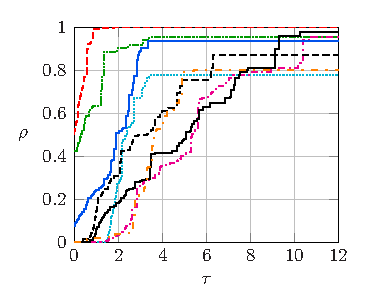
\includegraphics{lexample_fig1}
  \caption{Example figure using external image files.}
  \label{fig:testfig}
\end{figure}

\lipsum[51]

\section{Discussion of \texorpdfstring{{\boldmath$Z=X \cup Y$}}{Z = X union Y}}

\lipsum[76]

\section{Conclusions}
\label{sec:conclusions}

Some conclusions here.


\appendix
\section{An example appendix} 
\lipsum[71]

\begin{lemma}
Test Lemma.
\end{lemma}


\section*{Acknowledgments}
We would like to acknowledge the assistance of volunteers in putting
together this example manuscript and supplement.

\bibliographystyle{siamplain}
\bibliography{references}
\end{document}
